\documentclass[10pt,UTF8]{article}

\usepackage{geometry}

\usepackage{ctex}

\geometry{a4paper,scale=0.9}
\ctexset{today=old}

\usepackage{booktabs}

% \usepackage{times}  % 设置正文字体为 Adobe Times Roman
% \usepackage{mathptmx} % 只加载数学字体
% \renewcommand{\rmdefault}{cmr} % 恢复正文字体为 Computer Modern Roman
% \usepackage{lmodern} % Latin Modern 字体，兼容 Computer Modern 字体

% \usepackage{newtxtext}  % 设置正文为 TeX Gyre Termes (类似 Times)
% \usepackage{newtxmath}  % 设置数学字体匹配

\usepackage{fourier} % 设置正文字体为 Utopia
% \usepackage{eulervm} % 设置数学字体为 Euler
\setmainfont{Times New Roman} % 设置正文字体为 Times New Roman

\usepackage{bm} % 数学粗体（避免斜体被取消）

% \usepackage{makecell}
% \usepackage{multirow} % 表格多行合并

% \usepackage{graphicx} %插入图片的宏包
% \usepackage{subfigure}
% \usepackage{float} %设置图片浮动位置的宏包

\usepackage{amsmath}
% \usepackage{esint} % 提供更丰富的积分符号
% \usepackage{amssymb}
% \usepackage{mathtools}

\usepackage{physics}

% \usepackage{siunitx}
% % 关闭警告
% \ExplSyntaxOn
% \msg_redirect_name:nnn { siunitx } { physics-pkg } { none }
% \ExplSyntaxOff

% \usepackage{bussproofs} % 自然演绎推理树

% 交叉引用
% 关闭边框，设置颜色
\usepackage[colorlinks=true, linkcolor=darkgray, citecolor=teal,
urlcolor=blue]{hyperref}
% 使 \cref 和 \Cref 可用
\usepackage{cleveref}

\usepackage{bookmark}  % 生成 PDF 大纲

\allowdisplaybreaks[3]  % 允许换页

\usepackage{xcolor}

%%%%%%%%%%%%%%%%%%%%%%%% tcolorbox %%%%%%%%%%%%%%%%%%%%%%%%%%
\usepackage[most]{tcolorbox}

\newenvironment{tipBox}
{
  \begin{tcolorbox}[colback=green!5!white,colframe=green!75!black,parbox=false,before
  upper=\par,before lower=\par]}
  {
\end{tcolorbox}}

\newenvironment{conceptBox}
{
\begin{tcolorbox}[colback=blue!5!white,colframe=blue!75!black]}
  {
\end{tcolorbox}}

\newenvironment{theoremBoxNoIndent}
{
\begin{tcolorbox}[colback=yellow!5!white,colframe=yellow!75!black]}
  {
\end{tcolorbox}}

\newenvironment{definitionBox}
{
  \begin{tcolorbox}[colback=blue!5!white,colframe=blue!75!black,parbox=false,before
  upper=\par,before lower=\par]}
  {
\end{tcolorbox}}

\newenvironment{theoremBox}
{
  \begin{tcolorbox}[colback=yellow!5!white,colframe=yellow!75!black,parbox=false,before
  upper=\par,before lower=\par]}
  {
\end{tcolorbox}}
%%%%%%%%%%%%%%%%%%%%%%%%%%%%%%%%%%%%%%%%%%%%%%%%%%%%%%%%%%%%

%%%%%%%%%%%%%%%%%%%%% amsthm %%%%%%%%%%%%%%%%
\usepackage{amsthm}

\theoremstyle{definition}
\newtheorem{definition inner}{Definition}[section]
\newenvironment{definition}[1][]
{
  \begin{definitionBox}
  \begin{definition inner}[#1]\hfill\par}
    {
    \end{definition inner}
\end{definitionBox}}

\theoremstyle{definition}
\newtheorem{theorem inner}{Theorem}[section]
\newenvironment{theorem}[1][]
{
  \begin{theoremBox}
  \begin{theorem inner}[#1]\hfill\par}
    {
    \end{theorem inner}
\end{theoremBox}}

\theoremstyle{definition}
\newtheorem*{proof inner}{\textit{Proof}}
\renewenvironment{proof}[1][]
{
\begin{proof inner}[#1]\hfill\par}
  {\qed{}
\end{proof inner}}

\theoremstyle{plain}
\newtheorem{tip inner}{Tip}[section]
\newenvironment{tip}[1][]
{
  \begin{tipBox}
  \begin{tip inner}[#1]\hfill\par}
    {
    \end{tip inner}
\end{tipBox}}

\theoremstyle{remark}
\newtheorem*{remark}{\textit{Remark}}
%%%%%%%%%%%%%%%%%%%%%%%%%%%%%%%%%%%%%%%%%%%%%%

% \usepackage{tikz}
% \usetikzlibrary{graphs, graphdrawing}
% \usegdlibrary{trees, layered, force} % 可选布局算法

\usepackage{tkz-graph}
\usetikzlibrary{shapes.geometric} % 引入椭圆形状支持

\DeclareMathOperator{\Pa}{Parents} % Parents
\DeclareMathOperator{\Ch}{Children} % Children
\DeclareMathOperator{\De}{Descendants} % Descendants
\DeclareMathOperator{\Nd}{NonDescendants} % Non-descendants
\DeclareMathOperator{\An}{Ancestors} % Ancestors
\DeclareMathOperator{\MB}{MarkovBlanket} % Markov Blanket

\newcommand{\blue}[1]{{\color{blue!50!black}#1}} % 蓝色字体

\begin{document}

\part*{Bayesian Networks (BN)}

\section{Definition}

\begin{definition}[Bayesian Network]
  A \textbf{Bayesian Network (BN)} is a probabilistic graphical model
  that represents a set of variables and their conditional dependencies.
  \begin{itemize}
    \item It is a \textbf{directed acyclic graph (DAG)}.
    \item Every \textbf{node} represents a \textbf{random variable}
      and is associated with a \textbf{conditional probability table (CPT)}.
    \item The \textbf{Local Markov Property} holds: each random
      variable is conditionally independent of its non-descendants
      given its parents.
  \end{itemize}
\end{definition}

\subsection*{An example}

\begin{center}
  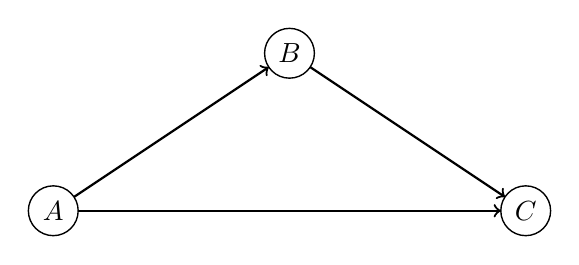
\begin{tikzpicture}
    \SetGraphUnit{2} % 设置节点间距
    \Vertex[L=$A$, x=0, y=0]{A}
    \Vertex[L=$B$, x=3, y=2]{B}
    \Vertex[L=$C$, x=6, y=0]{C}

    % 绘制有向边
    \Edge[style={->}](A)(B)
    \Edge[style={->}](A)(C)
    \Edge[style={->}](B)(C)
  \end{tikzpicture}
\end{center}

\subparagraph{Conditional Probability Tables (CPTs)}

\begin{equation*}
  \begin{array}{c c}
    \toprule
    A & P(A) \\
    \midrule
    1 & 0.2 \\
    2 & 0.5 \\
    3 & 0.3 \\
    \bottomrule
  \end{array}
  \qquad\qquad
  \begin{array}{c c c}
    \toprule
    A & B & P(B \mid A) \\
    \midrule
    1 & \text{T} & 0.7 \\
    1 & \text{F} & 0.3 \\
    2 & \text{T} & 0.4 \\
    2 & \text{F} & 0.6 \\
    3 & \text{T} & 0.9 \\
    3 & \text{F} & 0.1 \\
    \bottomrule
  \end{array}
  \qquad\qquad
  \begin{array}{c c c c c c c c c c c c c}
    \toprule
    A & 1 & 1 & 1 & 1 & 2 & 2 & 2 & 2 & 3 & 3 & 3 & 3\\
    B & \text{T} & \text{T} & \text{F} & \text{F} & \text{T} &
    \text{T} & \text{F} & \text{F} & \text{T} & \text{T} & \text{F} &
    \text{F} \\
    C & +1 & -1 & +1 & -1 & +1 & -1 & +1 & -1 & +1 & -1 & +1 & -1 \\
    P(C \mid A, B) & 0.8 & 0.2 & 0.5 & 0.5 & 0.6 & 0.4 & 0.3 & 0.7 &
    0.9 & 0.1 & 0.4 & 0.6 \\
    \bottomrule
  \end{array}
\end{equation*}

\subsection{The CPTs}

For a node without parents,
the CPT simply gives the prior distribution of the variable.

For a random variable \(X_i\) with parents \(\Pa(X_i)\), the
conditional probability table (CPT) specifies the probabilities
\(P(X_i \mid \Pa(X_i))\).

\bigskip

To be more specific,
let \(X\) be a node in the BN and
let the set of its parents \(\Pa(X) = \{ Y_1, Y_2, \ldots, Y_n \} \). Suppose:
\begin{itemize}
  \item \(\bm{Y} = (Y_1, Y_2, \ldots, Y_n)\) is a tuple of the
    \textbf{parents} of \(X\).
  \item \(\bm{y} = (y_1, y_2, \ldots, y_n)\) denotes a variable that
    takes values of \(\bm{Y}\).
\end{itemize}
The CPT of node \(X\) defines a multi-variable function as follows:
\begin{align*}
  f(x, \bm{y}) & := P(X = x \mid \bm{Y} = \bm{y})
  \\
  & = P(X = x \mid  \big \{ Y_1 = y_1, Y_2 = y_2, \ldots, Y_n = y_n \big \} ) \\
  & = P(X = x \mid \! \! \! \!
    \bigcup_{Y_j \, \in \, \Pa(X)} \! \! \! \! \! \!
  \big \{ Y_j = y_j \big \} ).
\end{align*}

\subsection{The Local Markov Property}

\begin{definition}[Conditional Independence]
  Let \(A\), \(B\), and \(C\) be three events.
  \(A\) is said to be \textbf{conditionally independent} of \(B\) given \(C\),
  denoted as \((A \perp B )\mid C\),
  if and only if:
  \[
    P(A \mid B \cup C) = P(A \mid C),
  \]
  or equivalently,
  \[
    P(A \cap B \mid C) = P(A \mid C) \cdot
    P(B \mid C)
  \]
\end{definition}

The Local Markov Property states that a node is conditionally
independent of its non-descendants given its parents.
Formally, for a node \(X\) in the BN\@:

\[
  X \perp \Nd(X) \; \; \mid \; \; \Pa(X),
\]
or more accurately,
\[
  X \; \perp \; \Nd(X) \setminus \Pa(X)
  \; \; \mid \; \; \Pa(X).
\]

This leads to the following equation:
\[
  P\big(X \mid \Pa(X) \cup \Nd(X)\big) =
  P\big(X \mid \Pa(X)\big)
\]

\section{Properties}

\begin{theorem}[Factorization Theorem / Chain Rule]
  Given a Bayesian Network with nodes
  \(\bm{U} = \{ X_1, X_2, \ldots, X_n \} \),
  the joint probability distribution of all random variables can be
  factorized as:
  \begin{align*}
    P(X_1 = x_1, X_2 = x_2, \ldots, X_n = x_n)
    & = \prod_{X_i \, \in \, \bm{U}} P\Big(X_i = x_i \mid
      \! \! \! \! \! \!
      \bigcup_{X_j \, \in \, \Pa(X_i)}
      \! \! \! \! \! \! \! \!
    \big \{ X_j = x_j \big \}  \Big)
  \end{align*}
  Given the values \(x_1, x_2, \ldots, x_n\),
  every factor on the RHS can be obtained from the CPT of a node.
\end{theorem}

\begin{proof}
  The proof is based on three preliminary points:
  \subparagraph*{1. General Chain Rule}
  For any random variables
  \( X_1, X_2, \ldots, X_n \),
  the joint probability distribution can be expressed as:
  \begin{align*}
    P(X_1, X_2, \ldots, X_n)
    & = P(X_1) \cdot
    P(X_2 \mid X_1) \cdot
    P(X_3 \mid \big \{ X_1, X_2 \big \} ) \cdots
    P(X_n \mid \big \{ X_1, X_2, \ldots, X_{n-1} \big \} ) \\
    & = \prod_{i=1}^{n} P\Big(X_i \mid
    \big \{ X_1, X_2, \ldots, X_{i-1} \big \} \Big)        \\
    & = \prod_{i=1}^{n} P\Big(X_i \mid
      \bigcup_{j=1}^{i-1}
    \big \{ X_j = x_j \big \}  \Big)
  \end{align*}
  \subparagraph*{2. The Local Markov Property}
  Let \(X\) be any node in the BN,
  \(\Nd(X)\) be the set of its non-descendants,
  and \(\Pa(X)\) be the set of its parents.
  \( \Pa(X) \subseteq \Nd(X) \).
  The property gives:
  \[
    P\big(X \mid \Nd(X)\big) =
    P\big(X \mid \Pa(X)\big)
  \]
  \subparagraph*{3. Topological Ordering}
  A DAG has at least one topological ordering,
  which means we can find an arrangement
  \(X_1, X_2, \ldots, X_n\) such that
  for any \(X_i\), \(\Pa(X_i) \subseteq \big \{ X_1, X_2, \ldots,
  X_{i-1} \big \} \).

  \bigskip
  Based on the above three points,
  let \(X_1,X_2,\ldots,X_n\) be in topological order,
  then we have:
  \begin{align*}
    P(X_1, X_2, \ldots, X_n)
    & = \prod_{i=1}^{n} P\Big(X_i \mid
    \big \{ X_1, X_2, \ldots, X_{i-1} \big \} \Big)   \\
    & = \prod_{i=1}^{n} P\Big(X_i \mid \Nd(X_i)\Big) \\
    & = \prod_{i=1}^{n} P\Big(X_i \mid \Pa(X_i)\Big)
  \end{align*}
\end{proof}

\section{Inference in a Bayesian Network}

\noindent
Some basic concepts:

\begin{itemize}
  \item \textbf{Query}: The variables we want to know about their distributions.
  \item \textbf{Evidence}: The variables and their observed values.
  \item \textbf{Hidden Variables}: The variables that are neither
    query nor evidence.
  \item \textbf{Goal}: Compute the conditional probability
    distribution of the query variables given the evidence.
\end{itemize}

\noindent
Different algorithms can be used for inference in Bayesian Networks, including:
\begin{itemize}
  \item \textbf{Exact Inference}: Enumeration, Variable Elimination,
    Belief Propagation.
  \item \textbf{Approximate Inference}: Monte Carlo methods,
    Variational Inference.
\end{itemize}

\subsection{Inference by Enumeration}

\subsubsection{The Method}

\begin{itemize}
  \item Query variable: \(X\)
  \item The tuple of evidence variables: \(\bm{E} = (E_1, E_2, \ldots, E_m)\)
  \item The tuple of observed values for evidence variables: \(\bm{e}
    = (e_1, e_2, \ldots, e_m)\)
  \item The tuple of hidden variables: \(\bm{H} = (H_1, H_2, \ldots, H_k)\)
  \item The tuple of values for hidden variables: \(\bm{h} = (h_1,
    h_2, \ldots, h_k)\)
\end{itemize}
\begin{align*}
  P(X = x \mid \bm{E}=\bm{e})
  & = \frac{P(X=x, \bm{E}=\bm{e})}{P(\bm{E}=\bm{e})}
  \\
  & = \alpha \cdot P(X=x, \bm{E}=\bm{e})
  \\
  & = \alpha \cdot \sum_{\bm{h}} P(X=x, \bm{H}=\bm{h}, \bm{E}=\bm{e})
  \\
  & = \alpha \cdot \sum_{h_1} \cdots \sum_{h_k} P(X=x, H_1=h_1,
  \ldots, H_k=h_k, \bm{E}=\bm{e})
\end{align*}
where \(\alpha \) is the normalization constant that can be found
after computing
\(P(X=x, \bm{E}=\bm{e})\) for all values of \(x\).

\noindent
The term \(P(X=x, \bm{H}=\bm{h}, \bm{E}=\bm{e})\) is a joint
probability distribution and can be computed using the Factorization Theorem.

\subsubsection{Time Complexity}

Suppose:
\begin{itemize}
  \item The BN has \(n\) nodes in total.
  \item Each random variable has at most \(d\) possible values.
  \item There are \(k\) hidden variables.
\end{itemize}

Further suppose reading from a CPT is \(O(1)\),
then computing each \(P(X=x, \bm{H}=\bm{h}, \bm{E}=\bm{e})\) takes \(O(n)\).

\subparagraph*{Conclusion}
The final time complexity is
\(O(n\cdot d^k)\),
or \(O(n\cdot d^n)\) as the evidence variables are usually only a few.

\subsection{Variable Elimination}

\subsubsection{Some Definitions}

\paragraph*{1. Factors}
A \textbf{factor} is a multi-variable function that maps some values taken
by a set of variables to a real number.
For example, a factor \(f(X, Y, Z)\) can be defined as:
\[
  f(x, y, z) = P(X=x \mid Y=y, Z=z)
\]

CPTs are also factors.

The order of parameters of a factor does not matter.
A variable is dependent on all other variables in the factors where it appears.
The dependences among variables are not directed.

\subparagraph*{Scope of a factor}
The \textbf{scope} of a factor is the set of variables that the
factor depends on.
For example, the scope of factor \(f(X, Y, Z)\) is \( \{X, Y, Z\} \).

\paragraph*{2. Pointwise product}
The \textbf{pointwise product} of two factors yields a new factor,
whose scope is the union of the scopes of the two factors.
Let \(f_1(X_1, X_2, \ldots, X_n, Z_1, Z_2, \ldots, Z_k)\) and
\(f_2(Y_1, Y_2, \ldots, Y_m, Z_1, Z_2, \ldots, Z_k)\) be two factors
with common variables \(Z_1, Z_2, \ldots, Z_k\).
The pointwise product \(f = f_1 \cdot f_2\) is defined as:
\[
  f(x_1, x_2, \ldots, x_n, y_1, y_2, \ldots, y_m, z_1, z_2, \ldots, z_k)
  := f_1(x_1, x_2, \ldots, x_n, z_1, z_2, \ldots, z_k) \cdot
  f_2(y_1, y_2, \ldots, y_m, z_1, z_2, \ldots, z_k)
\]

\paragraph*{3. Summing out}
Factors show the dependences among variables.
When a variable only appears in one factor,
we can conclude that it only depends on the variables in that factor.
Thus, we can \textbf{sum up} all possible values of that variable
to eliminate it from the factor.

Let \(f(X, Y_1, Y_2, \ldots, Y_n )\) be a factor.
The operation of \textbf{summing out} variable \(X\) from factor \(f\)
yields a new factor \(\phi \) defined as:
\[
  \phi(y_1, y_2, \ldots, y_n) := \sum_{x} f(x, y_1, y_2, \ldots, y_n)
\]

\subsubsection{Algorithm Steps}

Throughout the algorithm,
we maintain a set of factors.

\paragraph*{1. The initial set of factors}
The initial factors are the CPTs of all nodes in the BN\@.
\subparagraph*{Evidence Instantiation}
If a factor contains evidence variables,
we restrict the factor to the observed values.
For example, \(f(x, y, e) := P(X=x \mid Y=y, E=e)\),
and we have observed \(E=e^*\),
then we replace the factor \(f\) with \(f'(x, y) := f(x, y, e^*)\).

\paragraph*{2. Pointwise product and summing out}
Pick a hidden variable \(H\) to eliminate.
\begin{enumerate}
  \item Identify all factors \(f_1,f_2,\ldots,f_k\) that contain variable \(H\).
  \item Compute the pointwise product of these factors to get a new
    factor \(f\).
  \item Sum out variable \(H\) from factor \(f\) to get a new factor
    \(\phi \) that does not contain \(H\).
  \item Add factor \(\phi \) to the set of factors and remove
    \(f_1,f_2,\ldots,f_k\).
\end{enumerate}

\paragraph*{3. Repeat}
Repeat the above step until a factor containing only the query variable \(X\)
is obtained and no other factors contain \(X\).

\paragraph*{4. Normalization}
The remaining factor \(\tau(X)\) gives an unnormalized distribution
over \(X\).
Normalize it to get the final result:
\[
  P(X=x \mid \bm{E}=\bm{e}) = \frac{\tau(x)}{\sum_{x'} \tau(x')}
\]

\subsubsection{Time Complexity}

Suppose:
\begin{itemize}
  \item The BN has \(n\) nodes in total.
  \item Each random variable has at most \(d\) possible values.
\end{itemize}

A factor involving \(m\) variables has \(d^m\) entries.

The pointwise product of two factors with \(m_1\) and \(m_2\)
variables results in a new factor with at most
\(m_1 + m_2\) variables,
and takes \(O(d^{m_1 + m_2})\) time to compute.

Summing out a variable from a factor with \(m\) variables
results in a new factor with \(m-1\) variables,
and takes \(O(d^m)\) time to compute.

The bottleneck occurs when doing pointwise products or summing out.

\subparagraph*{Conclusion}
The time complexity is \(O(n\cdot d^{w+1})\),
where \(w\) is the treewidth of the graph.
In the worst case, \(w\) can be about \(n\).

\subsubsection{Another View of the Algorithm}

We use an example to illustrate the process of variable elimination,
to provide another perspective to understand the algorithm.

\begin{center}
  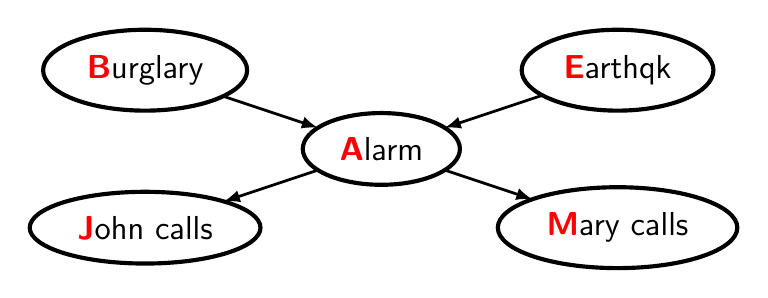
\begin{tikzpicture}
    % 定义颜色
    \definecolor{textred}{RGB}{255, 0, 0}
    % 自定义命令：首字母红色加粗
    \newcommand{\RedFirst}[1]{\textbf{\textcolor{textred}{#1}}}
    % --- 设置全局样式 ---
    \GraphInit[vstyle=Normal] % 初始化图风格

    % 重定义 VertexStyle (节点样式)
    \tikzset{VertexStyle/.style = {
        shape=ellipse,          % 形状：椭圆
        draw=black,       % 边框颜色
        fill=white,             % 填充颜色
        line width=1.5pt,       % 边框粗细
        inner sep=5pt,          % 内部文字边距
        align=center,           % 文字居中
        font=\large\sffamily    % 字体设置
    }}

    % 重定义 EdgeStyle (连线样式)
    \tikzset{EdgeStyle/.style = {
        ->,                     % 箭头
        >=latex,                % 箭头形状
        line width=1pt,         % 线条粗细
        color=black             % 线条颜色
    }}

    % --- 定义节点 (Vertices) ---
    % 使用绝对坐标 (x, y) 定位

    % 上层节点
    \Vertex[x=-3, y=1, L={\RedFirst{B}urglary}]{B}
    \Vertex[x=3,  y=1, L={\RedFirst{E}arthqk}]{E}

    % 中间节点
    \Vertex[x=0,  y=0, L={\RedFirst{A}larm}]{A}

    % 下层节点
    \Vertex[x=-3, y=-1, L={\RedFirst{J}ohn calls}]{J}
    \Vertex[x=3,  y=-1, L={\RedFirst{M}ary calls}]{M}

    % --- 定义连线 (Edges) ---
    \Edge(B)(A) % Burglary -> Alarm
    \Edge(E)(A) % Earthqk -> Alarm
    \Edge(A)(J) % Alarm -> John calls
    \Edge(A)(M) % Alarm -> Mary calls

  \end{tikzpicture}
\end{center}

Given observations that \(J=j\) and \(M=m\),
we want to compute the probability of burglary \(B\).
We start with the formula in the enumeration method:
\begin{align*}
  P(B \mid j, m)
  & = \alpha \cdot \sum_{e} \sum_{a}
  P(B, e, a, j, m) \\
  & = \alpha \cdot \sum_{e} \sum_{a}
  P(B) \cdot P(e) \cdot P(a \mid B, e) \cdot
  P(j \mid a) \cdot P(m \mid a)
  \qquad\text{by the Chain Rule} \\
  & = \alpha \cdot \sum_{e}
  P(e) \cdot \sum_{a}
  P(a \mid B, e) \cdot P(j \mid a) \cdot P(m \mid a) \\
  &\qquad\qquad P(B),\ P(e),\ P(a \mid B, e),\
  P(j \mid a),\ P(m \mid a) \text{ correspond to \(5\) factors.}\\
  & = \alpha \cdot P(B) \sum_{e}
  P(e) \cdot \sum_{a} f_1(B, e, a) \\
  &\qquad\text{\(3\) factors are merged. This is equivalent to
  performing pointwise products.} \\
  & = \alpha \cdot P(B) \sum_{e}
  P(e) \cdot \phi_1(B, e)
  \qquad\text{Variable \(A\) is summed out.}
\end{align*}

In the enumeration method,
we do not factor out the common factors.
In variable elimination,
we extract common factors to reduce redundant computations.

But different order of eliminating variables leads to different sizes
of intermediate factors,
which may result in different time cost when performing
pointwise products and summing out.
\begin{align*}
  P(B \mid j, m)
  & = \alpha \cdot \sum_{e} \sum_{a}
  P(B) \cdot P(e) \cdot P(a \mid B, e) \cdot
  P(j \mid a) \cdot P(m \mid a) \\
  & = \alpha \cdot P(B) \sum_{a}
  P(j \mid a) \cdot P(m \mid a) \sum_{e}
  P(e) \cdot P(a \mid B, e)
  \qq{\text{The summation order can be switched.}}
\end{align*}

Finding the optimal order of eliminating variables is NP-hard.
But there are some heuristics to find a good order
that usually works well in practice.
For example,
the \textbf{min-fill} heuristic chooses the variable
that minimizes the number of edges added to the graph
when the variable is eliminated.

\subsection{Rejection Sampling}

Rejection sampling is a Monte Carlo method for approximate inference.

\subparagraph*{Main idea}
Simulate the generation of a large number of samples,
reject those that do not match the observed Evidence,
and finally calculate the frequency of the query variable appearing
in the remaining samples.

\subsubsection{Algorithm Steps}

Assume we want to compute \( P(X_Q \mid X_E=\tilde{e}) \),
where \(X_Q\) is the query variable
and \(X_E=\tilde{e}\) is the evidence.

\subparagraph*{1. Topological sort}
Obtain the sorted sequence \(X_1, X_2, \ldots, X_n\),
where every node is behind its parents.

\subparagraph*{2. Samples generation}
In each sample, nodes are instantiated in topological order.
This guarantees that when generating \(X_i\),
its parents already hold concrete values,
thereby determining the distribution of \(X_i\) via its CPT\@.

\subparagraph*{3. Consistency check (rejection step)}
If the value of the evidence variable \(X_E\) in the generated sample
does not match the observed value, reject this sample (do not count it).
Note: reject the whole sample (including the parents generated).

\bigskip

Suppose we generate \(N\) samples (including both accepted and rejected ones):
\(S^{(1)}, S^{(2)}, \ldots, S^{(N)}\),
where each sample \(S^{(i)}\) is a tuple of values\@:
\(S^{(i)} = (x_{1}^{(i)}, x_{2}^{(i)}, \ldots, x_{n}^{(i)})\).
Suppose the query variable is \(X_Q\).
Then the query distribution can be approximated as:
\[
  P(X_Q = \hat{x} \mid X_E=\tilde{e}) \; \; = \; \;
  \frac{\displaystyle\sum_{i=1}^N \big[{x_Q^{(i)} = \hat{x}} \big]
  \cdot \big[{x_E^{(i)} = \tilde{e}} \big]}
  {\displaystyle\sum_{i=1}^N \big[{x_E^{(i)} = \tilde{e}} \big]}
\]
where \(\displaystyle\sum_{i=1}^N \big[{x_E^{(i)} = \tilde{e}} \big]\)
is the number of accepted samples.

\subsubsection{Problems}

Low efficiency:
when the evidence \(X_E=e\) is a rare event,
lots of samples are rejected, wasting a lot of time.

\subsection{Likelihood Weighting}

A directly improved version of rejection sampling.

\subparagraph*{Topological sort}
Same as in the rejection sampling.

\subparagraph*{Evidence instantiation}
Instead of randomly generating a value for the evidence variable \(E\),
we fix it to the observed value \(e\),
and continue to generate values for the following variables.

\subparagraph*{Weight}
The final sample is assigned a weight
\(w = P(E=e \mid \big \{
      \Pa(E) = \text{generated values for the parents of } E \big
\}) \).
By the definition, the weight can directly obtained from the CPT of \(E\).
If there are multiple evidence variables,
the final weight is the product of the weights calculated for each
evidence variable.

\bigskip

Suppose we generate \(N\) samples:
\(S^{(1)}, S^{(2)}, \ldots, S^{(N)}\),
where each sample \(S^{(i)}\) has a weight \(w^{(i)}\) and is a tuple of
values for all variables in the BN\@:
\(S^{(i)} = (x_{1}^{(i)}, x_{2}^{(i)}, \ldots, x_{n}^{(i)})\).
Suppose the query variable is \(X_Q\).
Then the query distribution can be approximated as:
\[
  P(X_Q = \hat{x} \mid E=e) \; \; = \; \;
  \frac{\displaystyle\sum_{i=1}^N w^{(i)} \cdot
  \big[{x_Q^{(i)} = \hat{x}} \big]}
  {\displaystyle\sum_{i=1}^N w^{(i)}}
\]

\subsection{Gibbs Sampling}

Gibbs sampling is a Markov Chain Monte Carlo (MCMC) method for
approximate inference.

\subparagraph*{Main idea}
Different from rejection sampling and likelihood weighting,
Gibbs sampling does not generate each sample independently.
Instead, it starts from an initial state (a sample),
and randomly walks through the state space
(generating a sequence of samples, where each sample is generated
based on the previous one).

\subsubsection{Algorithm Steps}

Suppose the BN has \(n\) variables.

\subparagraph*{1. Initial state}
Pick an initial state by fixing the evidence variables
to their observed values,
and randomly assigning values to all other variables.
Let the initial state be
\(S_1 = (x_1^{(1)}, x_2^{(1)}, \ldots, x_n^{(1)})\).

\subparagraph*{2. Sample sequence generation}
In each iteration, we update the value of one non-evidence variable
based on the current values of all other variables.
Let the \(i\)-th state (sample) be
\(S_i = (x_1^{(i)}, x_2^{(i)}, \ldots, x_n^{(i)})\).
To generate the next state \(S_{i+1}\):

\begin{enumerate}
  \item Pick a non-evidence variable. Suppose it is \(\blue{X_k}\).
  \item Compute the conditional distribution of \(X_k\)
    given the current values of all other variables:
    \[
      P\Big(\blue{X_k} \mid
        \big \{ X_1 = x_1^{(i)}, \ldots, X_{k-1} = x_{k-1}^{(i)},
      X_{k+1} = x_{k+1}^{(i)}, \ldots, X_n = x_n^{(i)} \big \} \Big)
    \]
  \item Sample a new value for \(\blue{X_k}\) from the above distribution.
    Let the new value be \(\blue{x_k^{(i+1)}}\).
  \item New state \(S_{i+1}\) is obtained by updating \(\blue{X_k}\):
    \[
      S_{i+1} = (x_1^{(i)}, \ldots, x_{k-1}^{(i)},
      \blue{x_k^{(i+1)}}, x_{k+1}^{(i)}, \ldots, x_n^{(i)})
    \]
\end{enumerate}

\subparagraph*{3. Derive the query distribution}
After generating a sufficiently large sample set,
the conditional distribution of the query variable can be
approximated by empirical frequency counts of its possible values.

\subsubsection{Some Optimizations}

\paragraph*{Markov Blanket}
When computing the conditional distribution of a variable \(\blue{X_k}\),
we do not need to consider all other variables.
In Bayesian Networks,
a variable is \emph{conditionally independent} of all other variables
given its \textbf{Markov Blanket}, which consists of:
\begin{itemize}
  \item Its parents.
  \item Its children.
  \item The other parents of its children (co-parents).
\end{itemize}
Thus, we only need to compute:
\begin{align*}
  & P\Big(\blue{X_k} \mid
  \big \{ \text{other variables} = \text{their previous values} \big \} \Big) \\
  &\qquad = P\Big(\blue{X_k} \mid
  \big \{ \MB(\blue{X_k}) = \text{their previous values} \big \} \Big) \\
  &\qquad \propto P\Big(\blue{X_k} \mid
  \big \{ \Pa(\blue{X_k}) = \text{their previous values} \big \} \Big) \cdot
  \! \! \! \! \!
  \prod_{C \, \in \, \Ch(\blue{X_k})} \! \! \! \! \! \! \! \! \!
  P\Big(C = \text{its previous value} \mid
  \big \{ \Pa(C) = \text{their previous values} \big \} \Big)
\end{align*}

\paragraph*{Burn-in}
It takes some time for the Markov chain to converge to
its stationary distribution.
To reduce the influence of the initial state,
we can discard the first several samples (for example, the first 1000 samples)
and only use the later samples to estimate the query distribution.
The discarded samples are called \textbf{burn-in} samples.

\paragraph*{Thinning}
In the generated sample sequence,
consecutive samples are highly correlated,
which is against the assumption of
\emph{independent identically distributed (i.i.d.)} samples
in statistical estimation.
To reduce the correlation between samples,
we can keep \(1\) sample every \(k\) samples
(for example, every \(100\) samples) and discard the others.

\subsubsection{Pros and Cons}

\paragraph*{Pros}
Usually more efficient than likelihood weighting,
especially in the presence of strong evidence in downstream variables.

\paragraph*{Cons}
Can be slow to converge,
especially when there exist multiple separated high-probability regions in the
state space.

\end{document}
